%%%% Proceedings format for most of ACM conferences (with the exceptions listed below) and all ICPS volumes.
%\documentclass[sigconf]{acmart}
%%%% As of March 2017, [siggraph] is no longer used. Please use sigconf (above) for SIGGRAPH conferences.

%%%% Proceedings format for SIGPLAN conferences 
% \documentclass[sigplan, anonymous, review]{acmart}

%%%% Proceedings format for SIGCHI conferences
%\documentclass[sigchi, review]{acmart}
\documentclass[sigchi]{acmart}

\settopmatter{printacmref=false} % Removes citation information below abstract
\renewcommand\footnotetextcopyrightpermission[1]{} % removes footnote with conference information in first column
\pagestyle{plain} % removes running headers

%%%% To use the SIGCHI extended abstract template, please visit
% https://www.overleaf.com/read/zzzfqvkmrfzn


\usepackage{booktabs} % For formal tables
\usepackage[utf8]{inputenc}

% Copyright
%\setcopyright{none}
%\setcopyright{acmcopyright}
%\setcopyright{acmlicensed}
\setcopyright{rightsretained}
%\setcopyright{usgov}
%\setcopyright{usgovmixed}
%\setcopyright{cagov}
%\setcopyright{cagovmixed}


% DOI
\acmDOI{}

% ISBN
\acmISBN{}

%Conference
\acmConference[]{}{}{}
\acmYear{}
\copyrightyear{}


%\acmArticle{4}
%\acmPrice{15.00}

% These commands are optional
%\acmBooktitle{Transactions of the ACM Woodstock conference}
%\editor{Jennifer B. Sartor}
%\editor{Theo D'Hondt}
%\editor{Wolfgang De Meuter}


\begin{document}
\title{Creating an Agent-Based Framework for Don't Starve Together}
%\titlenote{Produces the permission block, and copyright information}
%\subtitle{Extended Abstract}
%\subtitlenote{The full version of the author's guide is available as \texttt{acmart.pdf} document}


\author{Fábio Almeida}
\affiliation{
  \institution{Instituto Superior Técnico}
  \city{Lisboa}
  \state{Portugal}
}
\email{fabio.vieira.almeida@tecnico.ulisboa.pt}

\author{Rui Prada}
\affiliation{
  \institution{Instituto Superior Técnico}
  \city{Lisboa}
  \state{Portugal}
}
\email{rui.prada@tecnico.ulisboa.pt}

\author{Samuel Mascarenhas}
\affiliation{
  \institution{Instituto Superior Técnico}
  \city{Lisboa}
  \country{Portugal}
}
\email{samuel.mascarenhas@tecnico.ulisboa.pt}

% no short authors on top of page
\renewcommand{\shortauthors}{}

\begin{abstract}
Today's video games are striving to maintain high levels of fidelity.
The realistic graphical representation of virtual worlds is only betrayed by the lack of believability that in-game characters present.
To maintain the immersion created by exquisite graphics, characters must be able to create the illusion of life, which requires them to possess basic human traits like social awareness, reactivity, and active goal pursuit.
Some game genres, like role playing games, have seen this problem being addressed by using agency based characters.
However, survival games have not been subject to the same attention.
In this work, we address this issue by proposing a framework that allows developers to create characters based on agency models for survival games.
By making use of FAtiMA Toolkit, a fully fledged model for agency, and Don't Starve Together, a popular survival game, we've implemented and published such a framework with an example character, Walter.
Walter has been run and tested against a behaviour tree based agent.
\end{abstract}

\keywords{Artificial Intelligence, Non Playable Characters , Believable Characters, Survival Games}


\maketitle

\section{Introduction}

In recent years, the continuous improvement and development in computer graphics has pushed video games to new levels of graphical fidelity.
Graphical representations of virtual worlds have become increasingly more realistic, allowing players to experience new levels of immersion \cite{brown:immersion}.
Additionally, with the recent boom in virtual reality systems, players have never been so physically immersed in a game's virtual world.

The increases on fidelity and lifelikeness of the virtual world cause players to create expectations on the interactions they can have on the world.
This expectation applies not only to interactions with the virtual world itself, but is also extended to the interactions with the characters that compose the world, typically called Non Playable Characters (NPCs).

Computer and player controlled characters need to act in a believable manner so that the illusion of reality created by exquisite graphics and physics, the player's immersion, is not broken \cite{thrainsson:emotion-games}.
The lack of believability in NPCs can break the player's immersion and can provide a bad gameplay experience, given that the game's flow and player's immersion are key elements to the gameplay experience \cite{ijsselsteijn:userexperience}.
Reactivity, goals, emotions, and social competence are necessary traits NPCs need in order to be believable \cite{bates:emotioninagents}.

Some game genres, like Role Playing Games (RPGs), which are heavily dependent on player to NPC interaction, have received special attention on the creation of believable characters.
However, other game genres, like survival games, have not received such attention.

Survival games, a genre that has seen a rise in popularity recently, are often based in open world scenarios that can be procedurally generated.
Either single or multi-player, some survival games revolve around resource collecting, crafting, and management of the character's needs (hunger and thirst, mostly), while others are set in supernatural worlds with some elements of horror: monster infested worlds where players have to survive by defeating them.

%Their popularity can be justified for their ability in making experiences like surviving a night or overcoming a simple enemy fun.
More often than not, survival games lack a specific objective other than surviving in a harsh world for as long as possible.
However, survival games are trending among players and game developers alike, seeing great attention in the indie game scene.

Don't Starve \cite{games:dontstarve}, for example, is a single player survival game set on a procedurally generated world where players have to collect, craft, explore, and fight to survive.
With a day and night cycle, Don't Starve provides an interesting gameplay by combining mechanics for temperature, wetness, hunger, health, and sanity.
The introduction of sanity to the game's character provides a novelty factor among its peers, giving the character a human-like trait appropriate for a survival game, representing the strain put on the character by having to survive the harshness of a world with nothing to start with.

Following the trend for multiplayer survival games, Don't Starve has also been released as a multiplayer game under the name of Don't Starve Together (DST) \cite{games:dontstarvetogether}.
The game is identical to its predecessor, though it allows several players to join the same world.
The multiplayer nature of the game brings new challenges to players that can either cooperate or compete for survival.
In extreme cases, players can even attack and kill each other giving the game an extra challenge to overcome.

However, the game counts with no NPCs to accompany players in their journey for survival, making players dependent on each other for gameplay.
The few autonomous non-aggressive characters of Don't Starve Together present limited behaviour and are not subject to the same rules as the players (hunger, health, sanity, etc.).

The nonexistence of interesting and robust Artificial Intelligence (AI) for characters is not exclusive to Don't Starve Together.
Other survival games suffer from the same problem: the lack of collaborative AI for NPCs capable of creating believable characters.

As said before, on other game genres like RPGs, tools exist and have been used for the creation of AI controlled NPCs that take into account the character's believability \cite{guimaraes:cif-ck}\cite{afonso:agents-that-relate}\cite{ferreira:merchant-model}.
Usually empowered by social models, these tools have not yet been applied to survival games.

Many modern day video games are dependent on player to NPC interaction, and while
some degree of independent decision making is implemented through the use of AI techniques, it’s mostly based on combat and has no social concern whatsoever.
This lack of social ability in NPC can badly impact their believability and in turn affect the player's gaming experience.

While some work has been done to tackle the problem of believability in NPC, survival games however, have not been subject of this effort.

\section{Games, Immersion and Believability}

\begin{figure}
  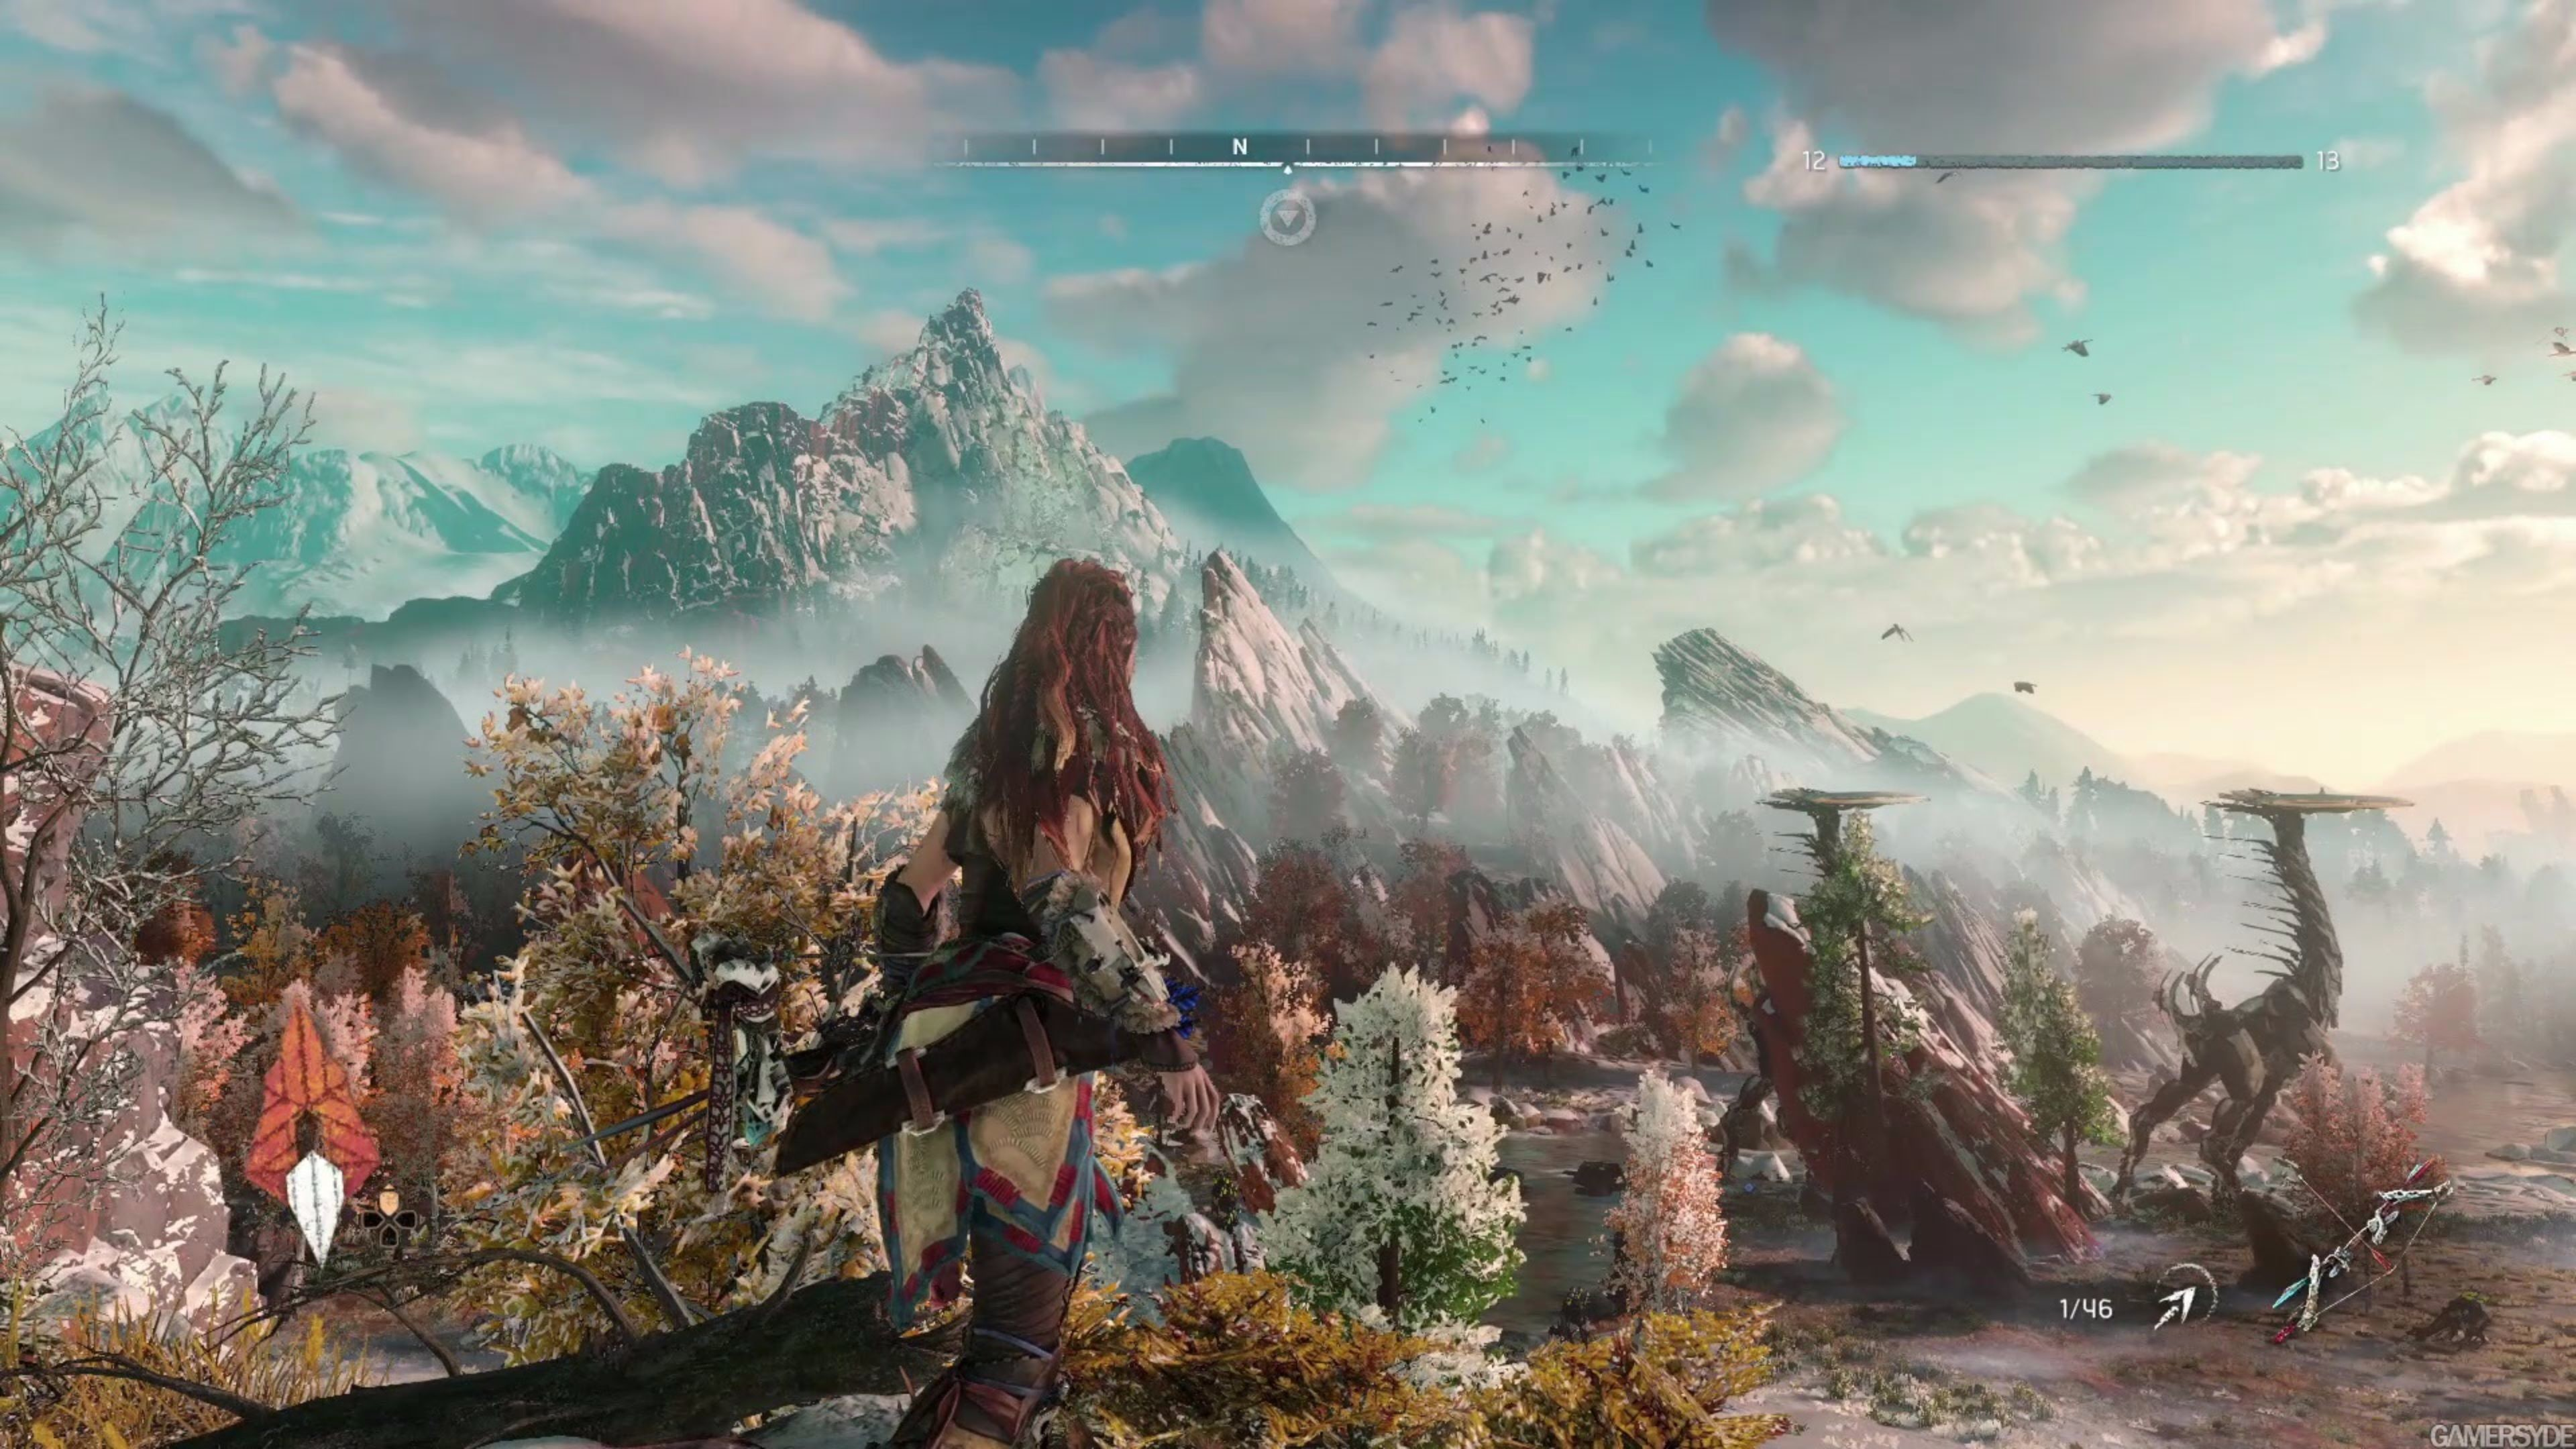
\includegraphics[width=0.49\textwidth]{./Images/horizon-zero-dawn}
  \caption{Horizon Zero Dawn exquisite graphics.}
  \label{fig:horizon}
\end{figure}

The increasing lifelikeness in video games gives players increasing expectations of better, meaningful experiences and interactions.
The world around the player is presented with exquisite graphics and increasing levels of fidelity, as proved by the recent title from Guerrilla Games, Horizon Zero Dawn \cite{games:horizon} (Figure \ref{fig:horizon}).

However, NPCs still have a lot of room for improvement.
Scripted behaviour and repetitive dialog, products of the lack of socially deep NPCs, can easily break the gaming experience of the player, due to reduced believability in the NPCs actions \cite{thrainsson:emotion-games}.
This contrast between the world and it's inhabitants may break the suspension of disbelief, one of the major factors needed to achieve a successful gaming experience \cite{ijsselsteijn:userexperience}.

The concept of believable characters has long been studied and explored in many different forms of art and media \cite{bates:emotioninagents}.
From the original Disney animators of the 1930's and the book later published on Disney's animations \cite{illusionoflife}, we can understand that in order to have believable characters we need to create the illusion of life.

\subsection{NPCs in games}

Most Triple-A video games make use of simple techniques to express NPC behaviour.
Finite State Machines (FSM), hierarchical FSM and behaviors trees are the most commonly used techniques in nowadays industry \cite{yannakakis:gameairevisited}.
However simple, they can achieve believable and expressive behaviours in the hands of skilled game designers.
These techniques can express logic, basic planning and  reactive behaviours.

Another advantage is that these techniques are deterministic, in other words, we can predict what can happen and then try to avoid problems.
Their major weakness, however, is their limited expressiveness, which can cause the realization of complex behaviors unmanageable.

In games like Assassin's Creed Unity \cite{games:assassinscreedunity} and Dragon Age Inquisition \cite{games:dragonageinquisition}, where there is a large number of NPCs, there is a tendency to make them reactive to the players instead of actively following their own goals.
In Dragon Age Inquisiton, many NPCs are present throughout the world doing absolutely nothing.
Sometimes, when the player approaches, she can overhear a conversation that is taking place between NPCs, usually directly related to the player, but these are always simple one or two sentences conversations and the player cannot interact with the NPC that is talking.

One can argue that, using current technology, it is impossible to make every single NPC socially aware and able to interact with the player.
However, even if we only look at the NPCs with which we can interact, their behaviour is repetitive and lacks depth.

Other games, such as The Elder Scrolls V: Skyrim \cite{games:skyrim}, have NPCs with occupations which they carry out during the day (the blacksmith will spend her day at the forge working), and houses where they return to during the night (almost every character will go to his home to have a meal and sleep).
These simple behaviours highly contribute to the character's believability as it provides the sense of having wants and needs. However, they still lack social ability.

If, for example, the player breaks into the house of a random NPCs, wakes her up and has a talk with her, she will ignore the fact that you just woke her up in the middle of the night in her locked house and proceed to have a completely normal conversation with the player.
The weirder part still, is that the player will be branded as a criminal and may face the city's guards upon exiting the house.
This lack of social ability can easily break the player's suspension of disbelief.

To address this problem we can make use of research based agency models for NPC control, as has been done in other works \cite{guimaraes:cif-ck-17}\cite{ferreira:merchant-model}\cite{evans:versu}\cite{mccoy:prom-week}\cite{sullivan:mismanor}\cite{mateas:facade}.

% \subsection{Socially empowered games}

% There are, however, some examples of socially focused games that are worth to mention not only for their value as games but also for their successful use of social architectures for NPCs.

% Blood and Laurels is a text-based interactive drama available in the App Store for the iPad\cite{evans:versu}.
% One of the game's appeal is its high re-playability due to the use of autonomous agents.
% The same episode can be played several times with different results.
% This is only made possible by making use of the Versu model.

% Prom Week is a social simulation game about the interpersonal lives of a group of high school students in the  week leading up to their prom\cite{mccoy:prom-week}.
% Gameplay in Prom Week involves solving level goals (such as making the class nerd, Zack, date a popular girl) within a limited number of turns by directing the characters to engage in social interactions.
% Which social games are available and how each changes the social state is managed by the game's AI system, Comme il Faut (CiF), which we discuss briefly below.
% Enabled by the social physics of CiF, each level's goal has innumerable solutions that maintain character believability.

% Mismanor is a social role-playing game where the player’s main form of interaction are actions that change the underlying social model \cite{sullivan:mismanor}.
% It makes use of an adaptation of the CiF architecture.
% In Mismanor, the player is guided through the dynamic story with quests that are chosen based on the actions the player has taken and their social standing with the character they are interacting with.
% Quests have multiple entry and exit points, giving the player more flexibility with how they choose to fulfill the request, with different consequences based on the path they have taken.

% In Façade\cite{mateas:facade}, the player is given almost no direction or role to play.
% The player can either play herself as the character or interpret the part of whomever she wishes.
% The drama takes place in a small simulated virtual world, the apartment of the married couple Grace and Trip.
% Façade was designed to deliver an experience that provides the player with 20 minutes of emotionally intense, undefined, dramatic action.
% The player's actions have a significant influence on how the story develops and how the drama ends.

\section{FAtiMA}
\label{section:fatima}

\begin{figure*}
  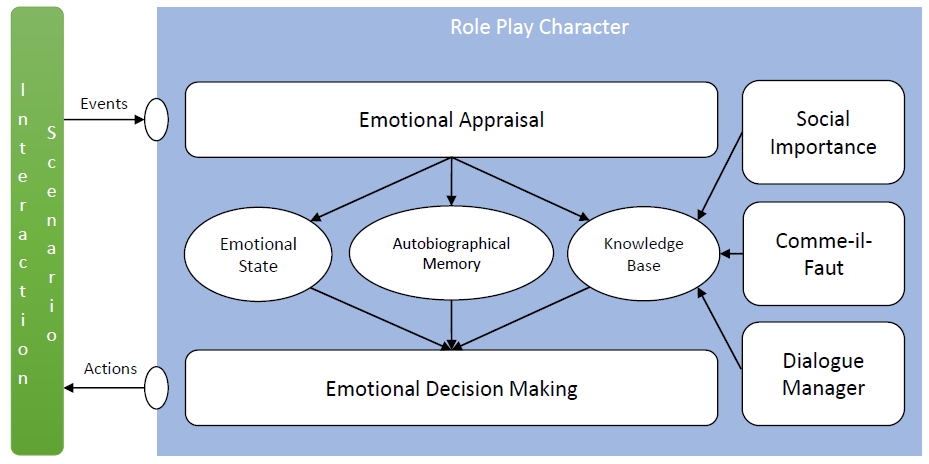
\includegraphics[width=0.7\textwidth]{./Images/rpc}
  \caption{The Role Play Character Asset aggregating all other assets to make an autonomous agent.}
  \label{fig:rpc}
\end{figure*}

Fearnot AffecTIve Mind Architecture (FAtiMA) is an agent architecture with planning capabilities designed to use emotions and personality to influence the agent's behaviour \cite{dias:fatima-modular}, and was developed to endow the characters in the serious game \textit{FearNot!} \cite{aylett:fearnot} with social intelligence.
It has been used successfully in different social scenarios (\cite{paiva:learning-by-feeling},\cite{rodrigues:i-can-feel-to}, \cite{aylett:intercultural-empathy}, and \cite{correia:sueca}) and it is based on appraisal theory \footnote{The theory that emotions are elicited by evaluations (appraisals) of events and situations \cite{roseman:appraisal}.}.

FAtiMA has a modular architecture where functionalities and processes are divided into modular independent assets.
This enables developers to use a lighter and simpler version of FAtiMA by adding the required assets, according to their necessities.
Therefore, behaviour and functionality are added by including assets in an agent's definition.
These assets will then implement the desired behaviours and functionalities.

FAtiMA comes with a set of predefined assets that can be used to define agents and their interactions\footnote{The toolkit is available at https://github.com/GAIPS-INESC-ID/FAtiMA-Toolkit.}.
Additionally, the developer can create its own assets that extend the toolkit's capabilities.
The available assets are:

\begin{description}
\item [Role Play Character Asset] \hfill

The Role Playing Character (RPC) Asset is an aggregation asset responsible for managing all the other assets that compose an agent.
It is also responsible for maintaining the agent's Emotional State and the agent's memory, which is divided in two components: a Knowledge Base and an Autobiographic Memory.

The Emotional State stores the current emotional state of the agent, defined by the Emotional Appraisal Asset, the Knowledge base stores the agent's beliefs, and the Autobiographic Memory stores the agent's recollections of past events and the emotions associated with such events.

\item [Emotional Appraisal Asset] \hfill

This asset appraises each event according to the OCC Theory of Emotions \cite{ortony:occ}.
Developer defined appraisal rules, determine how an agent evaluates certain events, determining the agent's Emotional State (which is kept by the RPC).

\item [Emotional Decision Making Asset] \hfill

The Emotional Decision Making Asset provides RPCs with decision making capabilities based on rules with logical conditions.
Allowing the agent to make multiple decisions at the same time, this asset makes use of the Knowledge Base and the Emotional State to decide which actions it decides to do.
FAtiMA handles this by making use of what it calls layers of decisions.
When the decision process is triggered, if a layer is provided, only actions for that layer are considered.

\item [Integrated Authoring Tool Asset] \hfill

This asset adds a Dialogue Manager that combines an hybrid solution between dialogue trees (a popular solution among game developers) and state machines to construct dialogues for agents.
The Dialogue Manager keeps the current state of dialogue, giving an agent (or player) every available option to choose from.

\item [Social Importance Asset] \hfill

The Social Importance Asset implements the \textit{SI} Dynamic Property, which represents the social relationship among two social entities A and B.
This representation, based on the status-power theory \cite{kemper:status-power}, gives information about how willing an agent is of complying with another agent's wishes.

\item [Comme il Faut Asset] \hfill

Based in the work described below, this asset allows developers to define Social Exchanges which, unlike single dialogue acts, are composed by sequential steps: initiate, answer, and finalize.
These steps represent an interaction between two agents.

\item [World Model Asset] \hfill

The World Model Asset gives developers a way to test the created agent in a simulated world where the consequences of each action is defined by the developer.
This asset is especially useful to test particular aspects of an agent.

\end{description}

It is important to note that the Comme il Faut (CiF) Asset can be used to complement the Social Importance Asset by giving an agent knowledge about social practices.
For example, while a boyfriend and father might have equally high social importance values, flirting is not an appropriate social practice when the target is the agent's father.
By defining flirting as a social exchange, the developer can define an additional condition to only activate this social exchange if the agent is attracted to the target.

% \subsection{Other Social Architectures}

% While we chose to use FAtiMA in our work, there are other socially aware models for agency being used nowadays that are worth to mention.

% \begin{description}
% \item[Comme il Faut] \hfill

% CiF is an AI system that enables authors to create interactive stories by specifying, not the complete narrative and all its ramifications but, high-level rules governing expected character behaviour given social situations \cite{mccoy:cif-social-story-worlds}.
% In CiF, characters use many attributes of the current social state, including the story of prior interactions, to decide how to engage in social exchanges with other characters.
% This architecture provides a rich social environment for characters to interact allowing the creation of dynamic and interactive stories.

% Social exchanges are the primary structure of representing knowledge in CiF \cite{mccoy:cif-authoring}.
% They consist in social interactions between characters that modify the social state of the participants.
% By using social exchanges and additional encoded social context, CiF lowers the authoring burden needed to create the social aspects of an interactive story by allowing the author to specify the rules and general patterns of how social interaction should take place.

% Characters' behaviour is chosen based on rules in a large rule database that depict normal social behaviour in a particular story world.
% These rules, in conjunction with the logic of a social world, a set of characters, and a series of scenario goals allows CiF to determine the desired action for each character.

% % More recently, a new version of CiF as been published and renamed to Ensemble.
% % Ensemble aims to empower NPCs with deeper interactivity and believability by modeling social states and behaviours for game characters \cite{treanor:ensemble}.
% % This extension presents a model of playable social dialogue called social practices.
% % Social practices increase the playability of character interactions and add interactivity at each stage of dialogue.

% \item[Versu] \hfill

% Versu model is based on Exclusion Logic \cite{evans:exclusion-logic}, a new deontic logic, and rests upon two kinds of objects: agents and social practices.
% To better make use of exclusion logic, the creators of Versu have also developed Praxis, a Domain Specific Language (DSL) used in the modeling of the social practices .

% Social practices describe a recurring social situation that may exist only for a short time (e.g. a conversation, a game, a meal) or can last much longer (e.g. a family, the moral community).
% These practices coordinate agents via the \textit{roles} they are playing and their main function is to describe the actions the agents can do in each situation.

% Social practices provide the agent with a set of suggested actions, but it is up to the agent himself to decide which action to perform, using utility-based reactive action selection (the utility is calculated in accordance with the agents beliefs, desires, personality quirks, and backstory).
% \end{description}

\section{Don't Starve Together}

Don't Starve Together is a multiplayer wilderness survival game developed by Klei Entertainment, where the players must survive as long as they can.
The players must face the harshnesses of a procedurally generated world that is actively trying to kill them, either by cooperating or competing with each other.
Each game can last an indefinite amount of time which is only determined by the players' ability to survive: the better you play the game, the longer you can last.

The game presents mechanics for hunger, health, temperature, wetness, day and night cycles, seasons, and sanity.
It also provides players with a monster infested world that try to kill the player's character.
The addition of multiplayer brings the possibility for social interaction among players, which contributes positively for the gameplay experience.

Moreover, the sanity mechanic itself is a differentiating factor from other games in the genre.
By providing a measurement of the characters' mental health, the game makes the characters more human and relatable.
A normal human being under such harsh environments would suffer physically but also mentally, and the sanity mechanic depicts just that.

For these reasons, the lack of AI controlled NPCs with believable behaviour, the ability to control and personalize the generated game world, and the possibility of introducing modifications into the game, we've decided to use this game as the target of our project.

\subsection{The Game}

A player's main concern is to keep the character's stats balanced throughout the game and find ways to survive the dangers each season brings.
To keep a steady supply of food and protection from the elements is as important as defending themselves from the monsters that will try to kill them.

Bellow is a list of the core game mechanics with a small description.
This list represents a compilation of key aspects we have to take into account while making a NPC for DST.

\begin{description}
	\item[\textbf{Health}] \hfill \\ When it reaches zero a character dies. It can be replenished by certain items and by eating appropriate food and will be lost while fighting and when in extreme conditions of temperature.
	\item[\textbf{Hunger}] \hfill \\ Will cause a character to start losing health when it reaches zero. It will gradually decrease over time and can be increased by eating food.
    \item[\textbf{Sanity}] \hfill \\ Represents the mental state of the character. Certain conditions will cause it to decrease (e.g. fighting or standing in the dark) while others can cause it to increase (e.g. eating certain foods or being around befriended \textit{pigmen}). When near zero will provoke hallucinations that can attack the character. 
	\item[\textbf{Temperature}] \hfill \\ In cases of extreme cold or heat the character will start to lose health over time. It can be kept in check with the use of craftable items like clothes and fires.
	\item[\textbf{Wetness}] \hfill \\ As the character gets herself wet it can drop held items, food in the inventory will spoil faster, and her temperature will also decrease. The use of umbrellas and appropriate clothing will prevent the wetness level from rising.
    \item[\textbf{Darkness}] \hfill \\ When in complete darkness a character will be attacked by the darkness creature. It is important to stay near a source of light during the night.
    \item[\textbf{Fighting}] \hfill \\ Either as a means of defense or of gathering food, fighting is a core game mechanic without which survival is impossible.
\end{description}

\subsection{Inner Workings}

Everything that exists in the world of Don't Starve Together is represented as an Entity, from the character the player controls, to the sounds the player hears.
These, in turn, are instances of \textit{prefabs} that can be accessed and edited in the Lua scripts used to make the \textit{mods}.
It is important to note that each entity is uniquely identified by a six digit Globally Unique Identifier (GUID).

By specifying and configuring its \textit{components}, \textit{stategraphs}, and \textit{brains}, the \textit{prefabs} define every entity in the game.
Each of these parts represent something different: \textit{components} represent what an entity does; \textit{stategraphs} represent how it looks; and \textit{brains} represent how it behaves.

When a \textit{prefab} is defined, it also configures its \textit{components}, for example, in the definition of the \textit{prefab} ``wood", which contains the \textit{component} ``fuel", there is also the configuration of this \textit{component} that, in comparison to the \textit{prefab} ``charcoal", has a lower level of ``fuel".
Effectively, \textit{components} describe functionalities that a given entity can have, and how that functionality works.
When an entity, either by a player's command or the \textit{brain}'s command, does a chop action, it is the \textit{components} of the held axe that determine how this action will be executed and trigger the appropriate animations and events.

While \textit{components} can be reused throughout different \textit{prefabs} (with different configurations), \textit{brains} are defined on a per \textit{prefab} basis.
Both butterflies and spiders share the ``locomotor" \textit{component}, but have distinct moving behaviours.

When defining the \textit{prefab}, if it is meant to have behaviour, an instance of a \textit{brain} is also defined and attached to the \textit{prefab}.
However, not all \textit{prefabs} have autonomous behaviour, and those that don't, don't have a \textit{brain}.
The \textit{brain} itself is a Behaviour Tree that is attached to an entity, telling it what to do, leaving the part of how to do it up to the entity's \textit{components}.

Using the Lua scripts, a \textit{modder} can create \textit{components}, \textit{stategraphs}, and \textit{brains}.
These can then be attached to existing \textit{prefabs} or new ones, also created by the \textit{modders}.

\section{Putting it together}

Now that we have explored both the game used as a scenario and the technology used to control the characters, it is time to look at how we connected both.
For the rest of this section, we'll present the implementation of the framework, explaining in full detail the decisions made.

The implementation itself consists in two modules: FAtiMA-DST, a Don't Starve Together \textit{mod}; and FAtiMA-Server, a C\# console application.
Both these modules have been made publicly available on the Github repository \href{https://github.com/hineios/FAtiMA-DST}{https://github.com/hineios/FAtiMA-DST}.
In the repository there is also a guide to help anyone develop an NPC for Don't Starve Together.
As shown in Figure \ref{fig:implementation}, the communication between the two modules is made using Hypertext Transfer Protocol (HTTP), which transfers JSON objects back and forth.

The choice of using HTTP communication arouse from a limitation we found while developing the initial proof of concept for this implementation.
Initially, we considered importing the FAtiMA Toolkit directly, as the loading of C\# Domain Specific Language (DLL) files into a Lua interpreter is possible.
However, as a security measure, the Lua interpreter embedded in DST blocks any importation of external libraries.
The inclusion of malicious libraries through the Steam Workshop would be a major security issue for both the company and the players.

As alternatives, we considered using textual files or a relational database that would act as a proxy between the modules, but we finally decided to use an HTTP connection as the game provided an easy way to make requests and register callback functions to handle the responses.
Due to the client-server nature of HTTP however, the FAtiMA-DST module continuously makes HTTP requests with JSON encoded data to the FAtiMA-Server module, which handles these requests yielding an appropriate response (also JSON encoded).
As a data-interchange format, JSON provides the necessary abstraction to exchange information between C\# objects and Lua tables.

\begin{figure*}
  \centering
    
\includegraphics[width=.8\textwidth]{./Images/implementation}
  \caption{A graphical representation of the implementation.}
  \label{fig:implementation}
\end{figure*}

\subsection{FAtiMA-Server}

The FAtiMA Toolkit is written in C\# and published as a set of DLL libraries.
Taking this into account, we decided to implement a simple server in C\#, capable of handling the HTTP requests made by FAtiMA-DST \textit{mod}.
This server contains a list of Role Play Character Assets that are uniquely linked with the agents running on the scenario.
Each request the server handles has an entity's (NPC) GUID, which is used to also identify a Role Play Character Asset.

Additionally, requests are divided into three categories: perceptions, events, and decisions.
Perception requests contain information on the NPC's state and field of vision, and happen periodically.
Event requests contain information on relevant world events, and happen whenever an event is triggered.
Decision requests trigger the decision process that tells the NPC what to do, and happen periodically.

If we consider the flow of information, the first two types (perception and event requests) represent a flow of information from the embodiment to the AI, while the third (decision requests) represents a flow of information from the AI to the embodiment.

When received, perception requests are translated into a series of Property-Changed events, that update the RPC's Knowledge Base.
Event requests will be translated to Action-End events and decision requests will trigger the RPC's decision process for the appropriate layer.

It is important to notice the limitations of using HTTP as the method of communication.
This form of communication makes it impossible for the AI to give direct actions to the embodiment, as we cannot send messages from the server to the client, only respond to client's requests.
As such, we have to rely on periodic requests made by the embodiment that will cause the AI to make a decision and respond with an action.

\subsection{FAtiMA-DST}

his module was implemented as a \textit{brain} for DST and is responsible to send perceptions to FAtiMA-Server and execute the actions it returns.
To achieve this, it sends a perception request to FAtiMA-Server two times a second, a decision request for behaviour every one and a half second, and a decision request for dialogue every ten seconds.
The values were tested and tweaked for the best compromise between behaviour and performance.

To send the perceptions to the FAtiMA-Server, it counts with a set of helper functions that extract the necessary information from surrounding entities.
A set of listeners relay information about events to the FAtiMA-Server, and a Behaviour Tree executes actions received from the FAtiMA-Server.

The Behaviour Tree makes use of the built-in Buffered Actions to execute the actions.
This provides a layer of abstraction over actions to handle all the locomotion details and appropriate verifications (e.g. it is only possible to chop a tree if an axe is held).

To handle the FAtiMA-Server commands, the tree contains two nodes: a node that executes actions (via buffered actions), and a node that handles the special behaviour of wandering.
The handling of dialogue is independent from the behaviour and is executed immediately without making use of the behaviour tree.

\section{Creating Walter}

As an example NPC, we've implemented a model based agent to demonstrate how one could use the set of available beliefs to create behaviour.
This example only makes use of FAtiMA's Dialogue Manager and Emotional Decision Making assets.

This example has been published to the Steam Workshop in the form of an AI companion, an NPC named Walter \footnote{The \textit{mod} public page can be found in this link: \href{http://steamcommunity.com/sharedfiles/filedetails/?id=1339264854}{http://steamcommunity.com/sharedfiles/filedetails/?id=1339264854}}.
On the \textit{mod}'s public page, a set of instructions can be found on how to run the character.
The page also contains links to the public repository where all the code for this framework can be found.

Currently, the framework counts with a total of forty eight beliefs and over fifty actions\footnote{The lists of beliefs and actions can be consulted in \href{https://github.com/hineios/FAtiMA-DST}{https://github.com/hineios/FAtiMA-DST}}.
By making use of the beliefs defined in the framework, we created a set of seventeen rules that give Walter its behaviour.

\subsection{Dialogue}

As far as speech goes, the current framework has some limitations.
Currently, there is no two-way communication, meaning that, although the agent can speak (through the use of text), the players will not be able to respond.
In Figure \ref{fig:axe-dialogue} we can see the execution of a speak action by the agent while he is executing another action.

\begin{figure}
  \centering
  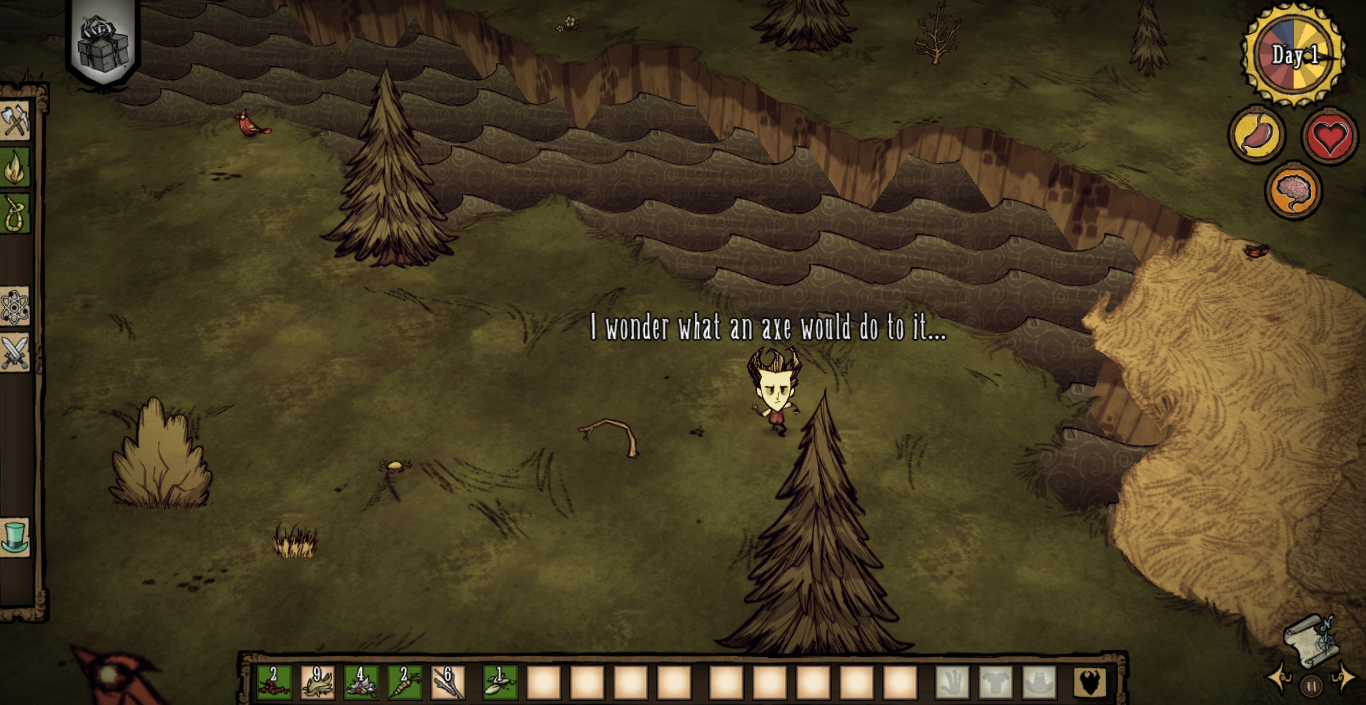
\includegraphics[width=0.49\textwidth]{./Images/axe-dialogue}
  \caption{Example of speak action.}
  \label{fig:axe-dialogue}
\end{figure}

\begin{figure}
  \centering
  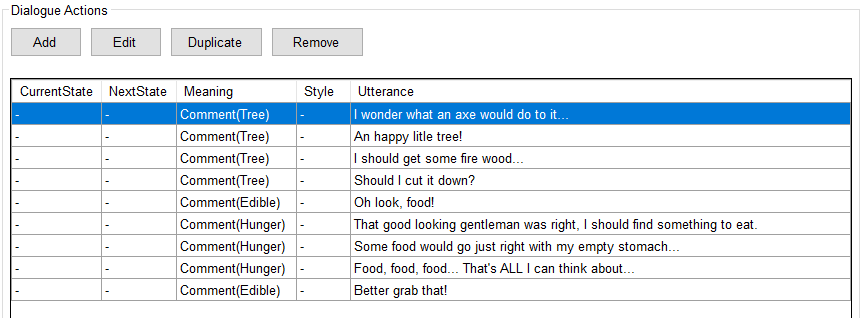
\includegraphics[width=0.49\textwidth]{./Images/dialogue-example}
  \caption{Walter's available dialogues.}
  \label{fig:dialogue-example}
\end{figure}

To make an NPC speak, the developer will need to create the available utterances using the Dialogue Editor as depicted in Figure \ref{fig:dialogue-example}.
Multiple utterances can be created with the same meaning, allowing for variety in the NPC's dialogue.
In Walter's example, several utterances have been added for each meaning.

To trigger these sentences, the developer also needs to add a rule with the appropriate layer to the decision making asset, as shown in Figure \ref{fig:dialogue-action-example}.
Here we can see, that in order for Walter to say a comment about hunger, his \texttt{Hunger} belief has to have a value lower than seventy.

\begin{figure}
  \centering
  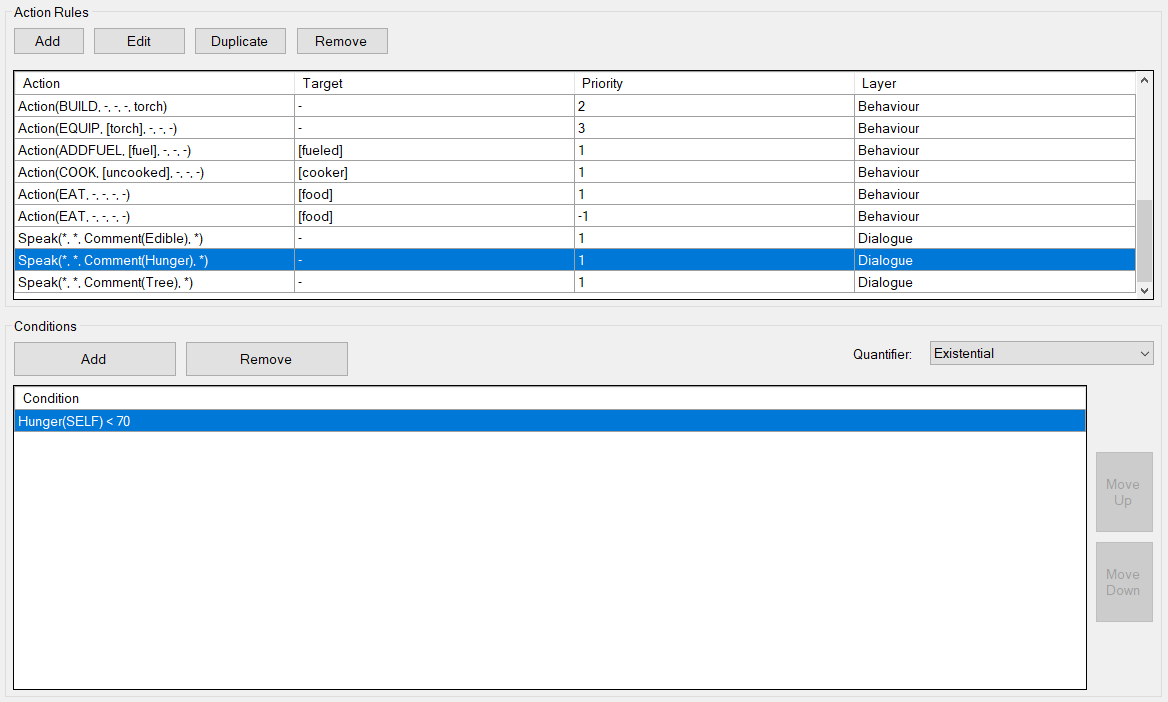
\includegraphics[width=0.49\textwidth]{./Images/dialogue-action-example}
  \caption{Walter's dialogue action rule.}
  \label{fig:dialogue-action-example}
\end{figure}

The addition of these sentences allows players to better understand the NPC's decision process.
By stating some random utterances about its current state, we can transmit the characters state of mind to the players.
These sentences can also be used to transmit the NPC emotional state, needs, and goals.

\subsection{Playing with Walter}

\begin{figure}
  \centering
  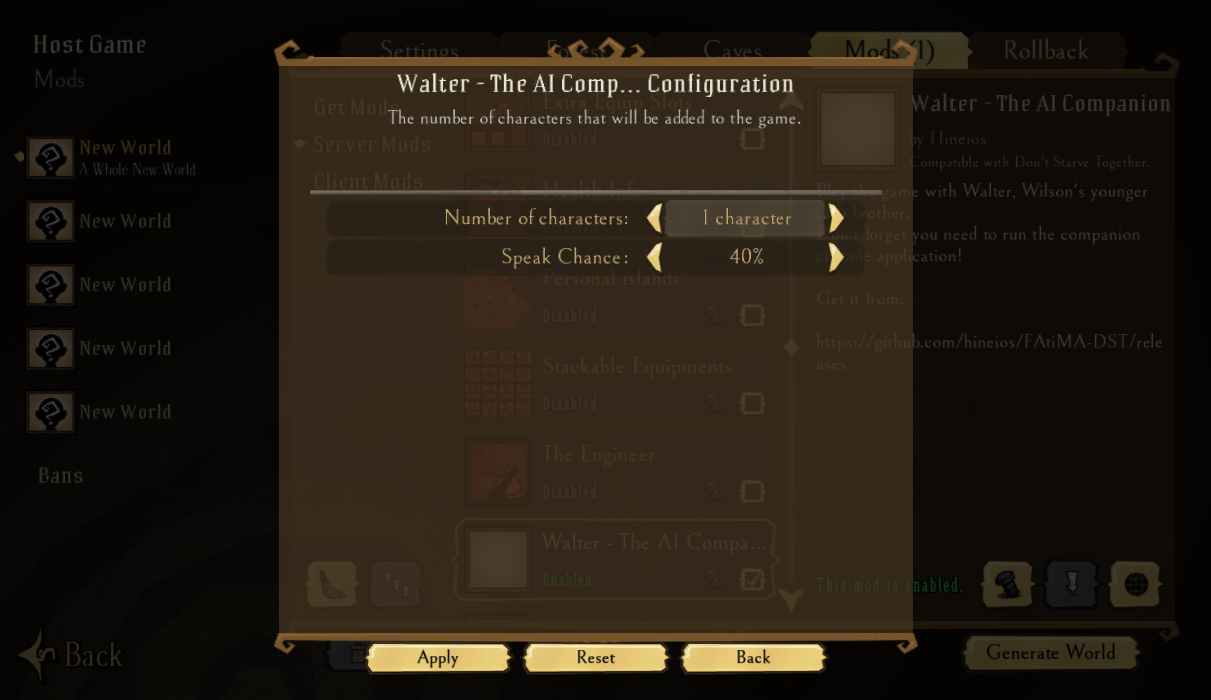
\includegraphics[width=0.49\textwidth]{./Images/mod-config}
  \caption{Configuration screen for FAtiMA-DST.}
  \label{fig:mod-config}
\end{figure}

In order to run our framework, players will have to run FAtiMA-Server by launching the console application available at the public repository.
FAtiMA-Server will automatically listen to HTTP requests on port 8080.
Then, before launching a game, the player will need to activate and configure the \textit{mod} as shown in Figure \ref{fig:mod-config}.
When the game is launched, the number of characters specified will spawn in the same place that players spawn.

\begin{figure}
  \centering
  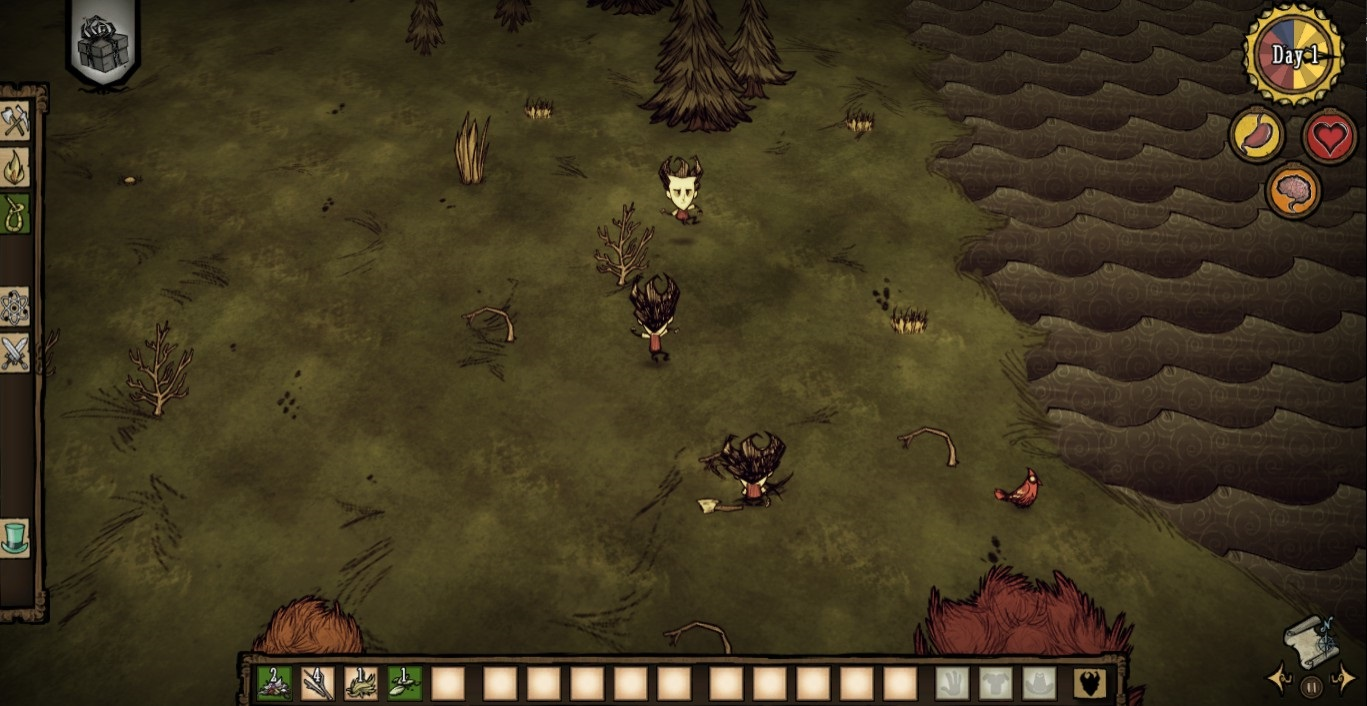
\includegraphics[width=0.49\textwidth]{./Images/multiple-agents}
  \caption{A player (center) playing the \textit{mod} with two FAtiMA controlled characters (top and bottom).}
  \label{fig:multiple-agents}
\end{figure}

In Figure \ref{fig:multiple-agents}, we can see an example of a player playing the game with two NPCs being controlled by FAtiMA.

\section{Evaluation}

We've successfully implemented a framework that enables developers to use an agency model, FAtiMA, to create NPCs for Don't Starve Together.
This was achieved through the implementation of a modification for DST and a companion console application.
As contributions resultant from this work we also count with a tutorial for creating NPCs and an example NPC.

\subsection{Walter - The AI Companion}

The example character we created to demonstrate the framework has been published in the Steam Workshop.
At the time of writing, with 48 days of existence, the \textit{mod} counts with 738 unique viewers and 128 subscribers.

While subscribers represent the number of people who've added the \textit{mod} to their game, it does not tells us how many of those have actually used the \textit{mod}.
The \textit{mod} also counts with 25 comments on the public page, mostly related to running the mod.

Although it has received no direct negative feedback, we believe that the necessity of running a separate console application has greatly impacted the community's acceptance and use of the \textit{mod}.
Additionally, to the best of our knowledge, no member of the community has used our framework to develop their own NPCs.

% \begin{figure}
%   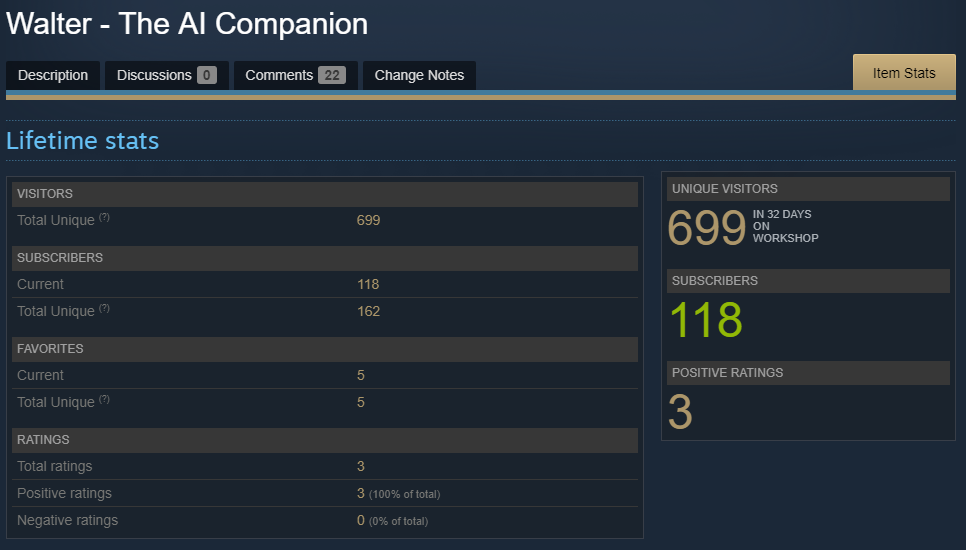
\includegraphics[width=.4\textwidth]{./Images/walter-stats}
%   \caption{Walter - The AI Companion \textit{mod} lifetime stats.}
%   \label{fig:walter-stats}
% \end{figure}

\subsection{Monte Carlo Tree Search Project}

As part of the Artificial Intelligence for Games course taught at Instituto Superior Técnico, a group of three students used our framework for their final project.
The project consisted in the implementation of the MCTS algorithm for the decision process of the agent.

Briefly, the Monte Carlo Tree Search (MCTS) algorithm is based in a random exploration of a state space.
By randomly (and rapidly) collecting data of the space state, the algorithm will gradually improve its knowledge of what the best next move is.

Unlike many other algorithms, MCTS does not run until an answer is found.
Instead, the usual approach consists in letting the algorithm run for some time (or a certain number of iterations) and then return the best possible action, in regard to the information collected so far.
The algorithm has proven to be especially good in problems where the space state has an high branching factor and many possible combinations, such as the Go game.

In this case, the implementation of the MCTS algorithm was achieved through the use of FAtiMA's Dynamic Properties.
The created Dynamic Property, called \texttt{MCTS}, will use current knowledge base and apply the MCTS algorithm.
The MCTS algorithm was let run for two thousand iterations (about twenty seconds) before returning a plan to act upon.

One of the main difficulties found during this use case was related to the random exploration of the state space.
As Don't Starve Together does not provide a way to simulate the resulting state of applying actions and FAtiMA did not have such functionality either (although it can now achieve this through the use of the World Model Asset), the group had to create their own simulator of the Don't Starve Together world.

This work, praises the versatility of our framework by demonstrating the ability to create a planning agent based on MCTS.
Although the group had to struggle with the world simulation, the end result was an NPC for DST with planning capabilities.

\subsection{Walter vs. Artificial Wilson}

As a means of evaluating the created NPC, we've run it and recorded how long it can survive.
Additionally, we compare it to an unpublished character for Don't Starve, Artificial Wilson.

Artificial Wilson, is the work of the anonymous \textit{modder} KingofTown and can be found in the public repository \href{https://github.com/KingofTown/DS-AI}{https://github.com/KingofTown/DS-AI}.

\subsubsection{Testing Conditions}

For each run of the characters, a new world was dynamically generated with equal sets of constraints for both characters.
The characters were then let run for as long as possible until their death.

As we said, Artificial Wilson was created for the original game, Don't Starve.
Therefore it is incompatible with Don't Starve Together because of the updates made to turn it into a multiplayer game.
However, the game mechanics and configurations remain the same.

As such, we can use the scenario configurator to generate equivalent worlds.
For this test, we considered the following restrains:

\begin{itemize}
	 \item \textbf{A world with no enemies}: all aggressive monsters have been removed from the game as well as the giants.
     \item \textbf{No random meteorological events}: apart from raining all other events have been disabled (like meteors,  frog rains, lightning storms, and wildfires).
     \item \textbf{No resurrection stones}: if the NPC dies, it stays dead.
     \item \textbf{No matting season for \textit{beefalos}}: during this season these, normally pacific creatures, will attack any character on sight.
     \item \textbf{No modifications}: apart from the necessary ones for running both characters.
     \item \textbf{Only one NPC and no players}: while in Don't Starve this does not apply, in Don't Starve Together the tests were run locally with no players present in the world.
\end{itemize}

These constrains will generate similar worlds for both Don't Starve and Don't Stave Together.
For each play-through of an agent, a new world is generated with these sets of constraints.
Each generated world is unique but complies to the specified set of constraints.

\subsubsection{The Results}

Each character has been run thirty times and the survival duration for each character is presented in Figures \ref{fig:days-survived-walter} and \ref{fig:days-survived-wilson}.

\begin{figure}
  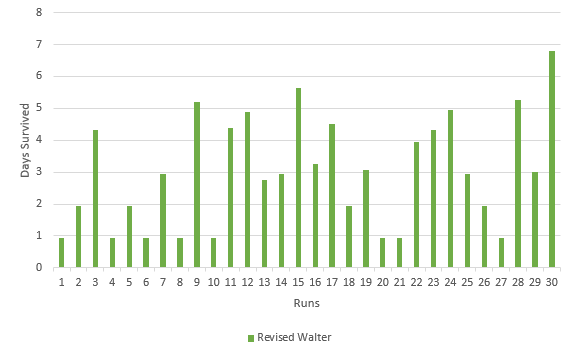
\includegraphics[width=.4\textwidth]{./Images/days-survived-walter-new-and-improved}
  \caption{Days survived for Walter.}
  \label{fig:days-survived-walter}
\end{figure}

\begin{figure}
  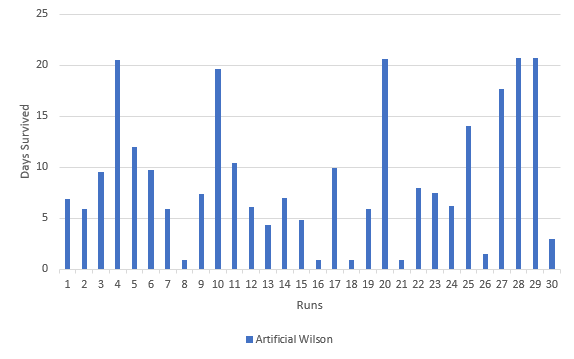
\includegraphics[width=.4\textwidth]{./Images/days-survived-wilson}
  \caption{Days survived for Artificial Wilson.}
  \label{fig:days-survived-wilson}
\end{figure}

Walter survived, on average, three days while Artificial Wilson survives, on average, eight point nine days.
The percentage difference of 99\% between both values can be explained by the detail put in each character's decision process\footnote{Percentage difference equals the absolute value of the change in value, divided by the average of the 2 numbers, all multiplied by 100. We then append the percent sign, \%, to designate the \% difference.}.

Walter is a model based agent with nineteen rules of decision.
Each of these rules has no decision process besides the character's ability to perform it (e.g. does the NPC has an axe equipped to cut down a tree?, does it have the required ingredients to build a fire?).

Artifical Wilson is based on the built-in behaviour trees.
The final behaviour tree counts with over seventy nodes and dozens of helper functions.
Embedded in the NPC's decision process are some planning capabilities and resource management (e.g. the NPC will ignore resources if she has already gathered enough of it), which Walter does not possess.

If we compare both characters to real human players, Walter has the ability of a newcomer who as never played the game, while Artificial Wilson could be compared to a returning player who played the game for a couple dozen of times\footnote{This comparison has been based on the writers' experience with the game}.

For each character we've recorded not only their survival time but also their cause of death.
In Table \ref{tab:cod} you can see a summary for both characters.

\begin{table}[htb]
	\centering
    \caption{Artificial Wilson and Walter cause of death summary.}
    \label{tab:cod}
    \begin{tabular}{ | p{0.2\linewidth} | p{0.1\linewidth} | p{0.2\linewidth} | p{0.1\linewidth} | }
        \hline 
        \multicolumn{2}{|c|}{Artificial Wilson} & \multicolumn{2}{|c|}{Walter} \\ \hline 
        CoD & Times & CoD & Times \\ \hline
        Cactus & 2 & Darkness & 17 \\ \hline
        Cold & 5 & Hunger & 13 \\ \hline
        Darkness & 10 & & \\ \hline
        Hunger & 13 & & \\ \hline
    \end{tabular}
\end{table}


\section{Conclusions}

The use of Behaviour Trees and Finite State Machines, the most commonly used techniques in today's industry, provide skilled game designers with the ability to create somewhat complex behaviour.
However, these techniques can quickly become an authoring burden.
Having to manage hundreds of behaviour nodes or states is no simple task.
Furthermore, grasping the context of social interaction will often be left out of the NPC's behaviour.

Focusing on survival games, we've noticed how these games will often lack the presence of NPCs, and when they are present, they can break the player's immersion by not being subject to the same rules as the players.
This, allied to the fact that many survival games rely on multiplayer interaction in order to keep interesting, has motivated us to create a platform that allows developers to create believable NPCs with interesting behaviour for survival games.

In order to make believable NPCs we need them to possess certain human-like traits: social awareness, active goal pursuit, and reactivity, for example.
By incorporating FAtiMA's capabilities into a commercial survival game we've been able to realize a platform that allows developers to create NPCs with social ability and planning capabilities.

We've chosen Don't Starve Together for its multiplayer nature, its ability to configure the world we play in, the possibility of including our own modifications to the game natively, and for its sanity mechanic.
A novelty among its peers, the sanity mechanic represents the character's mental health, another component that enhances the player's immersion by giving the character a human trait.

Then we implemented the \textit{mod}, FAtiMA-DST, and the console application, FAtiMA-Server, that allow us to run AI powered NPCs in DST.
As an example and proof of concept, we've also created Walter, a model based NPC that was published in the Steam Workshop.

Additionally, the platform has been successfully used to implement a planning agent using the MCTS algorithm.
By creating a new Dynamic Property, the developers were able to create an agent using FAtiMA and run it in DST.

In order to evaluate our work, we've compared our example agent, Walter, with Artificial Wilson, an agent created using the in-game's behaviour trees by an anonymous \textit{modder}.
Although Walter's performance is poor when compared to Artificial Wilson, the discrepancy can be justified due to the difference in the size of both implementations.
While Walter counts with nineteen rules of decision, Artificial Wilson counts over seventy nodes in its behaviour tree.

This dissertation provides the ground work for future developments in the creation of NPCs for survival games, in particular for Don't Starve Together.
It is our belief that with an equal effort, Walter's behaviour would at least match the performance of Artificial Wilson with the added value of social awareness, emotional responses, and active goal pursuit.

\subsection{Future Work}

As this work stands, it allows the creation of NPCs for Don't Starve Together.
However, the platform has great room for improvement.

\begin{itemize}
\item Two-way communication.
Currently, the platform allows the NPC to talk and make remarks on the world.
However, the player is not able to respond and talk back to the NPC.
Either by allowing chat responses or by adding an additional component to the game's interface, the interaction with the NPC could be greatly improved.

\item Add more beliefs.
Expanding the character's available beliefs will enable us to create more complex behaviour.
However, only by adding behaviour to NPCs, will we understand which beliefs are effectively necessary.

\item Improve Walter.
As a proof of concept Walter plays its role as expected.
Nonetheless, Walter is a simple model based agent that does not make full use of FAtiMA's capabilities.
Although the framework is fully prepared to support FAtiMA, the character does not benefit from all the capabilities FAtiMA might grant to a virtual agent. By incorporating additional assets into the RPC's definition, like the Emotional Appraisal Asset or the Social Importance Asst, Walter could be further improved.

\item Reduce the burden of running FAtiMA's characters in DST.
As it stands, players have to run a console application in parallel with the game for the platform to work properly.
It is our belief that by removing this requirement, more players would be able to play with NPCs that make use of our platform.
Ideally, this would be done by incorporating FAtiMA's DLLs into the embedded Lua interpreter that DST comes with.
However, this would require some sort of collaboration with the game developers, Klei Entertainment.
Alternatively, a public server could be set up to host the FAtiMA-Server component.

\item Add an additional layer of decision.
Players can express feelings through the use of gestures.
Gestures are animations that represent different states of mind the player may be feeling (some of the available gestures are ``annoyed", ``bye", ``angry", ``joy", ``dance", and ``sad").
The addition of this capability to the platform would be a great improvement as far as believability goes for created NPCs.

\item Add more composed actions to the platform.
Currently the only composed behaviour incorporated in the platform is the wander behaviour.
The addition of combat behaviour, utilization of chests, structure placement helpers, and others, would greatly improve an NPC's capabilities.

\item Different NPCs running different RPCs.
For each NPC there should be an ability to specify the RPC to be loaded.
This would enable the creation of richer scenarios by using characters with different characteristics, goals, reactions, dialogues, among others.

\end{itemize}


\bibliographystyle{ACM-Reference-Format}
\bibliography{bibliography}

\end{document}
